\problemname{Exploring Delsjön}
\noindent

Olle likes to take walks in the woods around Delsjön. In the woods, there are $N$ glades, and $N-1$
trails that connect them. It is possible to travel between every pair of glades using one or more trails.
It takes exactly one minute to travel along one trail to another glade. 
The forest can only be entered and exited via glades that have exactly one trail connecting the glade
to the rest of the forest. There are $K$ such glades, and we will call them \textit{exit glades}.
Olle has taken enough walks to know the time it takes to walk between every pair of the $K$ exit glades.

He wonders if this information is enough to map out the forest. Your task is to find a possible layout of the
forest that is consistent with Olle's information, using at most $2000$ glades. More exactly, you should first
decide on the number of glades $G$, and then decide the $G-1$ trails connecting the glades. The layout should
be such that glade $1$ is the first exit glade, glade $2$ is the second exit glade in the same order as the input, up to $K$.
It must also be possible to walk between every pair of glades in your layout.

\section*{Input}
The first line of input contains the integer $K$ ($2 \leq K \leq 1000$), the number of exit glades.

Then follow $K$ lines, the $i$:th describing the distances between exit glade $i$ and the other exit glades. Each line $i$ will contain
$K$ integers, $d_{i,1}, d_{i,2}, \dots, d_{i,K}$ ($1 \leq d_{i,j} \leq 1000$), each $d_{i,j}$ meaning that it takes $d_{i,j}$ 
minutes to get from glade $i$ to $j$. Note that these distances are symmetric: $d_{i,j}=d_{j,i}$ for all $i,j$.

It is guaranteed that the input is created such that there always exists a layout where $G \leq 1000$.

\section*{Output}
First, print an integer $G$ ($K \leq G \leq 2000$), the number of glades in your layout.

Then, print $G-1$ lines, each containing two integers $a,b$ ($1 \leq a,b \leq G$), meaning that there
is a trail between glade $a$ and $b$. Glade $1$ should be the first exit glade, glade $2$ the second
exit glade and so on.

If your layout of Delsjön is consistent with the information given above and it is possible to travel between
every pair of glades using one or more trails, it will be accepted.

\section*{Scoring}
Your solution will be tested on a set of test groups, each worth a number of points. Each test group contains
a set of test cases. To get the points for a test group you need to solve all test cases in the test group.

\noindent
\begin{tabular}{| l | l | p{12cm} |}
  \hline
  \textbf{Group} & \textbf{Points} & \textbf{Constraints} \\ \hline
  $1$    & $50$       & There is a solution with $G \leq 100$. \\ \hline
  $2$    & $50$       & No additional constraints. \\ \hline
\end{tabular}

\section*{Explanation of Sample 1}
One possible way that Delsjön could look like is shown below: 
\begin{center}
  \begin{figure}[h]
    \centering
    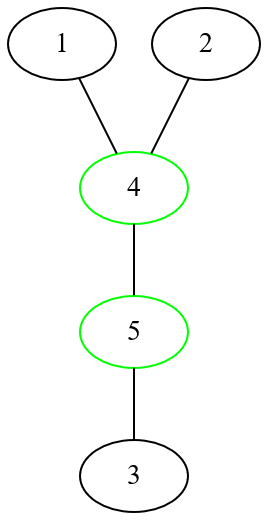
\includegraphics[width=0.2\textwidth]{sample-1.png}
  \end{figure}
\end{center}
The black glades are exit glades. You can verify that the distances 
between each pair of exit glades matches those in the input.

\section*{Explanation of Sample 2}
Given the distances of sample 2, Delsjön could look like what is shown below: 
\begin{center}
  \begin{figure}[h]
    \centering
    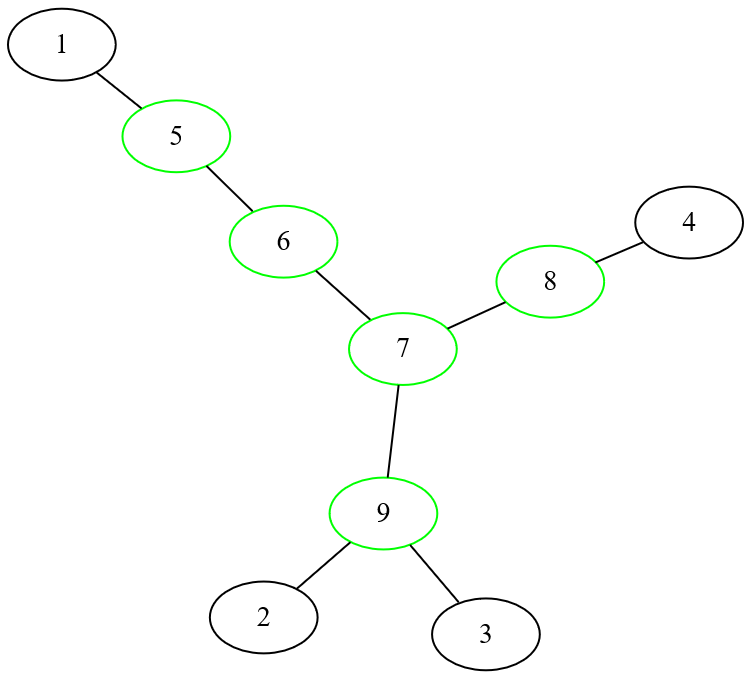
\includegraphics[width=0.4\textwidth]{sample-2.png}
  \end{figure}
\end{center}
